\documentclass[beamer]{standalone}
\definecolor{printred}{RGB}{215,25,28}
\usepackage{lmodern}
\usepackage{tikz}
\usetikzlibrary{patterns}
\begin{document}
\newcommand{\drawstencil}[2]{%
  \draw[darkgray, thick, pattern=north west lines, pattern color=gray] (#1-1, #2) rectangle (#1+2, #2+1);
  \draw[darkgray, thick, pattern=north west lines, pattern color=gray] (#1, #2-1) rectangle (#1+1, #2+2);
  \draw[darkgray, thick, pattern=north east lines, pattern color=gray](#1, #2) rectangle (#1+1, #2+1);
}
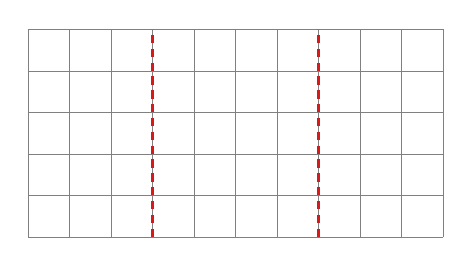
\begin{tikzpicture}[x=1.5em,y=1.5em]

  \draw[step=1, gray, very thin] (0,0) grid (10, 5);

  \drawstencil{3}{2}

  \onslide<2> {
    \draw[printred, densely dashed, very thick] (3,0) -- (3,5);
    \draw[printred, densely dashed, very thick] (7,0) -- (7,5);
  }
\end{tikzpicture}
\end{document}
